\documentclass[preprint,11pt]{elsarticle}
\usepackage[T1]{fontenc}
\usepackage{lmodern}
\usepackage{amsmath,amssymb,booktabs,array,graphicx}
\usepackage[margin=25mm]{geometry}
\usepackage[colorlinks=true,citecolor=blue,urlcolor=blue,linkcolor=blue]{hyperref}
\pdfstringdefDisableCommands{\def\corref#1{}}
\graphicspath{{figures/}}
\journal{Physical Communication}
\bibliographystyle{elsarticle-num}
\setlength{\emergencystretch}{2em}
\begin{document}
\begin{frontmatter}
\title{Residual-noise calibration in off-grid OFDM:\\Leakage bias, temporal correlation, and cyclic-prefix controls}
\author{Yuxiao Kuang\corref{cor1}}
\ead{b24041416@njupt.edu.cn}
\author{Wenqing Liu}
\ead{b24041901@njupt.edu.cn}
\author{Wenjie Li}
\ead{b25041315@njupt.edu.cn}
\cortext[cor1]{Corresponding author.}
\address{Nanjing University of Posts and Telecommunications, Nanjing, China}
\begin{abstract}
Pilot-residual noise calibration couples OFDM receiver decisions to the
assumed channel subspace: excluded signal energy is counted as noise.
We quantify when this leakage dominates calibration error and test the
reconstruction gain available from changing the calibration source.
Gaussian quadratic-form analysis separates squared leakage bias from
finite-window variance, identifies their crossover for independent blocks,
and quantifies the effect of temporally correlated gains. Delay-offset and subspace sweeps distinguish
the benefit of suppressing leakage from the cost of losing residual noise
dimensions. With 16 pilots and a 12-dimensional integer subspace, a separated
fractional-delay profile at 20~dB gives a pooled noise estimate approximately
8.78 times the thermal variance. In an independent paired experiment with
900 groups per condition, an established cyclic-prefix difference statistic
replaces residual calibration in the same continuous-delay receiver. At
20~dB SNR, normalized channel-estimation error improves by 2.98~dB and
4.25~dB for separated and closely spaced paths, respectively; paired 95\%
bootstrap intervals are [2.57, 3.34] and [3.97, 4.52]~dB. A finite-burst
waveform check verifies fractional-delay cancellation, and the experiment
preserves the dependence between cyclic-prefix and FFT noise. Together,
the analysis and controlled intervention distinguish calibration gaps that
benefit from further averaging from those that call for a different noise
source or channel representation.
\end{abstract}
\begin{keyword}
OFDM \sep noise variance estimation \sep fractional delay \sep channel estimation \sep cyclic prefix
\end{keyword}
\end{frontmatter}

% Analytical core. Requires amsmath, amssymb and a natbib-compatible citation setup.
% Invoke \CoreDiscussion after the experimental/results sections.
\section{Introduction}
\label{sec:introduction}

Noise calibration affects both the strength of channel denoising and the
choice of a channel model in pilot-assisted orthogonal frequency-division
multiplexing (OFDM). When no independent noise measurement is available, a
receiver can estimate the noise variance from the portion of its pilot
observations left unexplained by an assumed channel subspace. This economical
approach couples calibration to the channel representation because unexplained
signal components enter the same residual energy as receiver noise. Increasing
the number of calibration blocks can therefore make a noise estimate more
repeatable without making it more accurate.

This distinction matters when a short integer-delay representation is used for
a channel with fractional path delays. The residual then contains channel
energy outside the selected subspace. Increasing the subspace dimension, however,
leaves fewer residual degrees of freedom for estimating noise. These effects
create a trade-off among channel approximation, calibration variance, and
observation cost. They also complicate the interpretation of downstream
performance. A change in channel-estimation error may reflect a
better representation, a different noise estimate, or a change in model order.

Established methods already address continuous channel parameters and unknown
statistics. Parametric OFDM receivers avoid an integer-delay restriction
\cite{hansen2018iterative}; variational line-spectrum estimation represents
continuous-parameter uncertainty and learns noise statistics
\cite{badiu2017valse}. Newtonized pursuit and its multiple-snapshot extension
provide further ways to refine continuous parameters
\cite{mamandipoor2016nomp,zhu2019mnomp}. These methods motivate a specific
diagnostic question: how much residual calibration error can additional
observations reduce, and how much requires a change in the signal model?

We quantify when residual calibration becomes dominated by channel leakage
and how temporal correlation changes the useful averaging window. The
projected channel covariance separates persistent bias, receiver-noise
fluctuations, and correlated leakage fluctuations. Their relative sizes give
a model-conditioned crossover between sampling-dominated and bias-dominated
calibration. Controlled OFDM comparisons then connect this distinction to
channel reconstruction: changing the channel representation and changing the
noise source address different parts of the error. A paired experiment
substitutes cyclic-prefix (CP) calibration within the same continuous-delay
receiver, using the existing waveform and preserving its noise dependence.
The resulting diagnostic identifies when additional averaging is useful and
when signal cancellation or a different channel representation is required.

\section{Related work}
\label{sec:related}

\subsection{Noise information and channel denoising}
Risk-based denoising offers an established alternative to assuming a known
channel covariance. Upadhya et al.\ use Stein's unbiased risk estimate to choose
linear and nonlinear OFDM channel estimators \cite{upadhya2016risk}. In their
accessible author preprint, the simulation setup estimates noise from 500 blank
OFDM carriers. This differs from estimating noise from a small residual
subspace of the pilots also used for channel estimation. Comparing these
settings requires distinguishing the denoising rule from the amount and source
of its noise information.

The CP provides noise information from samples already present in the waveform.
Cui and Tellambura estimate the power delay profile and noise variance from
the repeated signal structure; their Eq.~(15) gives a direct CP--tail
difference statistic \cite{cui2006pdpnoise}. Their simplified channel model
rounds delays to integers and assumes synchronization and blockwise channel
invariance. Here that established statistic serves as a calibration-source
control: a conservative delay bound selects a clean repetition interval, a
finite-burst waveform check verifies fractional-delay cancellation, and paired
receiver comparisons retain the dependence between CP and FFT noise. This
separates the source of noise information from the denoising rule that uses it.

\subsection{Continuous parameters and multiple observations}
Continuous-delay modeling has a direct counterpart in line-spectrum
estimation. Newtonized orthogonal matching pursuit (NOMP) alternates detection
with refinement of sinusoidal parameters and uses a noise-dependent stopping
criterion \cite{mamandipoor2016nomp}. Its multiple-snapshot extension, MNOMP,
uses observations with shared frequencies and snapshot-dependent amplitudes
\cite{zhu2019mnomp}. For OFDM, Gao et al.\ exploit common delay structure and
spatial and temporal correlations \cite{gao2014superresolution}. These
approaches use shared channel structure across observations, whereas residual
energy pooling shares a scalar noise statistic. The distinction matters when
comparing observation budgets and attributing gains to calibration.

Unknown noise and continuous parameters can also be inferred jointly. VALSE
maintains approximate frequency distributions, selects a model order, and
updates the noise and gain statistics \cite{badiu2017valse}. Hansen et al.\
incorporate parametric channel estimation into an iterative OFDM receiver that
exchanges soft information with a decoder and represents dense channels through
a virtual channel impulse response \cite{hansen2018iterative}. These methods
establish joint continuous-parameter and noise inference; the calibration
question here concerns the consequences of retaining a fixed residual subspace.

Subsequent variational formulations extend uncertainty-aware inference to
multidimensional spectra \cite{zhang2020mdvalse} and noise variances that vary
across sensors or snapshots \cite{zhang2021heteroscedastic}. For underwater
acoustic OFDM, Wan et al.\ jointly estimate frequency offset, continuous-delay
channels, and noise statistics while exchanging information with a decoder;
their initialization also uses pilot-only VALSE \cite{wan2022jccdvalse}.
These developments reinforce the distinction between learning nuisance
parameters within a channel model and examining the consequences of fixing an
imperfect calibration subspace.

Table~\ref{tab:priorwork} organizes these precedents by the information they
use. Our contribution is the quantitative connection between a fixed
subspace's leakage, the averaging window, and the reconstruction gain obtained
by changing the calibration source. Standard Gaussian quadratic-form identities
provide the analytical basis. A specified orthogonal matching pursuit
(OMP)/variable-projection receiver provides the controlled intervention, and
a separate paper-equation VALSE implementation examines joint inference in
the pilot domain.

\begin{table}[t]
\centering
\caption{Closest prior approaches and the calibration question examined here.
The rows distinguish information use, rather than numerical performance.}
\label{tab:priorwork}
\small
\renewcommand{\arraystretch}{1.12}
\begin{tabular}{@{}>{\raggedright\arraybackslash}p{0.23\linewidth}>{\raggedright\arraybackslash}p{0.33\linewidth}>{\raggedright\arraybackslash}p{0.38\linewidth}@{}}
\toprule
Approach & Established mechanism & Relation to this study \\
\midrule
Risk-based denoising \cite{upadhya2016risk} & SURE selects channel denoisers;
the author preprint uses 500 blank carriers for noise estimation. & Separates
the denoiser from the quantity and source of noise observations. \\
CP calibration \cite{cui2006pdpnoise} & Direct CP--tail differences cancel
repeated signal samples. & Supplies the established statistic for a paired
calibration-source substitution with fractional delays. \\
NOMP/MNOMP and common-delay OFDM \cite{mamandipoor2016nomp,zhu2019mnomp,gao2014superresolution}
& Continuous parameters and shared geometry improve channel fitting. &
Distinguishes sharing channel structure from pooling residual energies. \\
VALSE and iterative OFDM receivers \cite{badiu2017valse,hansen2018iterative,wan2022jccdvalse}
& Joint inference learns continuous parameters, model order, and noise;
iterative receivers also use decoder information. & Motivates the pilot-domain
joint-inference check and fixes the information boundary of the receiver controls. \\
\bottomrule
\end{tabular}
\end{table}

\section{System model}
\label{sec:system}

\subsection{OFDM observations and delay convention}
Consider a single-antenna OFDM link with an even number $N$ of subcarriers. Let
$q_k=k$ for $0\leq k<N/2$ and $q_k=k-N$ otherwise, and set $f_k=q_k/N$ in cycles
per base-rate sample. The frequency response in block $t$ is
\begin{equation}
 H_{t,k}=\sum_{j=1}^{J}g_{t,j}\exp(-\mathrm{i}2\pi f_k\tau_j),
 \qquad k=0,\ldots,N-1,
 \label{eq:channel}
\end{equation}
where $\tau_j$ is measured in sample periods and delays remain fixed over a
calibration window. The path gains are zero-mean proper complex Gaussian with
covariance $\mathbf P=\operatorname{diag}(p_1,\ldots,p_J)$ and
$\sum_jp_j=1$. This normalization applies to the ensemble; individual channel
realizations are not rescaled.

There are $M$ equally spaced pilots of value one at indices $k_m=mD$, where
$D=N/M$. After division by the known pilots, the observations satisfy
\begin{equation}
 \mathbf y_t=\mathbf B\mathbf g_t+\mathbf n_t,
 \quad B_{mj}=\exp(-\mathrm{i}2\pi f_{k_m}\tau_j),
 \quad \mathbf n_t\sim\mathcal{CN}(\mathbf0,v\mathbf I_M).
 \label{eq:pilotmodel}
\end{equation}
Noise is independent across blocks and of all gains. The scalar
$v$ is the variance per complex pilot observation and is constant within the
window. Under the normalization above, the nominal subcarrier SNR is $1/v$,
excluding CP and pilot overhead. True delays, powers, and $v$ are used for data
generation and explicitly identified oracle references; practical estimators
do not receive them.

The numerical setting uses $N=64$, $M=16$, and a nominal integer-delay window
of length $L=12$. For fractional delays, replacing a negative frequency by its
unsigned FFT index changes the continuous-delay phase, so the signed-frequency
convention matters. Pilot delay atoms have a period of $M$ samples in this
setting, and the predefined search interval $[0,12]$ lies within one such
period. All generators and estimators use the same convention.

\subsection{Waveform assumptions and calibration windows}
For a useful symbol and its CP, the ideal transmitted waveform is
\begin{equation}
 s_t(u)=\frac{1}{\sqrt N}\sum_{k=0}^{N-1}X_{t,k}
             \exp(\mathrm{i}2\pi f_ku),
 \qquad -N_{\rm CP}\leq u<N.
 \label{eq:waveform}
\end{equation}
Adjacent CP-extended symbols occupy separate rectangular intervals. With ideal
delayed paths, exact synchronization, constant gains during the received
symbol, and $N_{\rm CP}\geq\max_j\tau_j$, CP removal and a unitary FFT give
the multiplicative response in \eqref{eq:channel}. To check finite-CP
consistency for ideal paths, the waveform audit applies linear delays to a
finite oversampled burst rather than a circular shift to each symbol
separately. The rectangular symbol boundaries do not form a globally bandlimited
analog waveform. Transmit/receive filtering, frequency offsets, Doppler, and
radio-frequency impairments are outside this model.

The main calibration experiment holds path geometry and noise variance fixed
while drawing independent gains for each block; a separate analysis allows
stationary temporal correlation. Independent fading blocks are not taken to be
consecutive OFDM symbols, because the observation duration needed to obtain
them depends on channel coherence. Only the first block is the target of
channel estimation and data detection. The other
blocks supply scalar calibration statistics unless a method is explicitly
defined to fit shared channel parameters.

\section{Analytical characterization of residual calibration}
\label{sec:analysis}

\subsection{Fixed subspaces and conditional moments}
Let $\mathbf A\in\mathbb C^{M\times L}$ contain the pilot responses of integer
delays $0,\ldots,L-1$, with $L<M$. For the comb pilots,
$\mathbf A^{\mathrm H}\mathbf A=M\mathbf I_L$. Define
\begin{equation}
 \mathbf Q=\mathbf I_M-\frac{\mathbf A\mathbf A^{\mathrm H}}{M},
 \quad d=M-L,\quad
 \mathbf z_t=\frac{\mathbf A^{\mathrm H}\mathbf y_t}{M},
 \quad R_t=\mathbf y_t^{\mathrm H}\mathbf Q\mathbf y_t.
 \label{eq:projection}
\end{equation}
$\mathbf Q$ is a fixed Hermitian projector with rank $d$. For a general
full-rank pilot basis, the projector is instead
$\mathbf I_M-\mathbf A(\mathbf A^{\mathrm H}\mathbf A)^{-1}\mathbf A^{\mathrm H}$;
the residual identities below remain valid. Pooling $T$ blocks gives
\begin{equation}
 \widehat v_T=\frac{1}{Td}\sum_{t=1}^{T}R_t.
 \label{eq:vhat}
\end{equation}

First condition on the noiseless observations
$\boldsymbol\mu_t=\mathbf B\mathbf g_t$. For proper complex Gaussian noise,
expanding $R_t$ into its deterministic, linear-noise, and quadratic-noise
terms yields
\begin{align}
 \mathbb E[R_t\mid\boldsymbol\mu_t]
   &=vd+\|\mathbf Q\boldsymbol\mu_t\|^2,\label{eq:conditionalmean}\\
 \operatorname{Var}(R_t\mid\boldsymbol\mu_t)
   &=v^2d+2v\|\mathbf Q\boldsymbol\mu_t\|^2.
 \label{eq:conditionalvariance}
\end{align}
The linear term has variance $2v\|\mathbf Q\boldsymbol\mu_t\|^2$;
the quadratic term has variance $v^2\operatorname{tr}(\mathbf Q^2)=v^2d$.
Their covariance is zero because centered Gaussian third moments vanish.
Since receiver noise is independent across blocks,
\begin{align}
 \mathbb E[\widehat v_T\mid\{\boldsymbol\mu_t\}]
  &=v+\frac{\sum_t\|\mathbf Q\boldsymbol\mu_t\|^2}{Td},
  \label{eq:poolconditionalmean}\\
 \operatorname{Var}(\widehat v_T\mid\{\boldsymbol\mu_t\})
  &=\frac{Tv^2d+2v\sum_t\|\mathbf Q\boldsymbol\mu_t\|^2}{T^2d^2}.
  \label{eq:poolconditionalvariance}
\end{align}
If the signal belongs to the assumed subspace, all projected means vanish.
Then $\sum_tR_t/v\sim\operatorname{Gamma}(Td,1)$, so
$\mathbb E[\widehat v_T]=v$ and
$\operatorname{Var}(\widehat v_T)=v^2/(Td)$. These statements remain true
for correlated gains when the subspace is correct, as the residual contains
receiver noise alone. Increasing $L$ reduces $d$, so a wider delay window
increases calibration variance even without mismatch.

\subsection{Ensemble leakage bias and Gaussian variance}
To average over channel realizations, define
\begin{equation}
 \mathbf C_s=\mathbf B\mathbf P\mathbf B^{\mathrm H},\qquad
 \mathbf S=\mathbf Q\mathbf C_s\mathbf Q,\qquad
 \mathbf C=\mathbf S+v\mathbf Q,\qquad
 b=\frac{\operatorname{tr}(\mathbf S)}{d}.
 \label{eq:leakagecovariance}
\end{equation}
Here $\mathbf S$ is the covariance of the signal remaining after projection;
$b\geq0$ is its residual energy per retained complex dimension. Since
$\mathbf Q^2=\mathbf Q$,
$\operatorname{tr}(\mathbf S)=\operatorname{tr}(\mathbf Q\mathbf C_s)$.
The projected observation is proper Gaussian with covariance $\mathbf C$,
possibly singular in the ambient pilot space. Diagonalizing this covariance
expresses its squared norm as a weighted sum of independent unit-mean
exponential variables, giving
\begin{equation}
 \mathbb E[R_t]=\operatorname{tr}(\mathbf C),\qquad
 \operatorname{Var}(R_t)=\operatorname{tr}(\mathbf C^2).
 \label{eq:singlemoments}
\end{equation}
The mean identity requires the stated second moments, whereas the variance
identity also uses proper Gaussian gains. For independent blocks,
\begin{align}
 \mathbb E[\widehat v_T]&=v+b,\label{eq:bias}\\
 \operatorname{Var}(\widehat v_T)
 &=\frac{\operatorname{tr}(\mathbf S^2)
          +2v\operatorname{tr}(\mathbf S)+v^2d}{Td^2}.
 \label{eq:independentvariance}
\end{align}
Pooling reduces variance around $v+b$ but leaves $b$ unchanged. For fixed
channel power and geometry, the relative bias $b/v$ increases with SNR.
These quantities separate thermal-noise estimation error from residual
signal-model error and can be computed before Monte Carlo simulation.

\subsection{Correlated calibration blocks}
Consider stationary Gaussian gains with a real autoregressive coefficient
$0\leq\rho\leq1$:
\begin{equation}
 \mathbf g_{t+1}=\rho\mathbf g_t+\sqrt{1-\rho^2}\,\mathbf w_t,
 \quad \mathbf g_1,\mathbf w_t\sim\mathcal{CN}(\mathbf0,\mathbf P),
 \label{eq:ar1}
\end{equation}
where the innovations are mutually independent and independent of receiver
noise. Thus
$\mathbb E[\mathbf g_t\mathbf g_u^{\mathrm H}]=\rho^{|t-u|}\mathbf P$.
For $t\ne u$, the residual cross-covariance is
$\rho^{|t-u|}\mathbf S$. The proper Gaussian fourth-moment identity gives
\begin{equation}
 \operatorname{Cov}(R_t,R_u)
   =\rho^{2|t-u|}\operatorname{tr}(\mathbf S^2).
 \label{eq:crosscovariance}
\end{equation}
Pairing the two cross-block factors in the expansion of
$\mathbb E[R_tR_u]$ produces the trace of the cross-covariance times its
Hermitian transpose; the within-block pairing cancels the product of means.
Summing all diagonal and off-diagonal terms yields
\begin{equation}
 \operatorname{Var}(\widehat v_T)=
 \frac{T\operatorname{tr}(\mathbf C^2)
 +2\operatorname{tr}(\mathbf S^2)
   \sum_{h=1}^{T-1}(T-h)\rho^{2h}}{T^2d^2}.
 \label{eq:correlatedvariance}
\end{equation}
The expectation remains \eqref{eq:bias}. To show which part of the variance
is affected by correlation, set
$a_T=T+2\sum_{h=1}^{T-1}(T-h)\rho^{2h}$. Then
\begin{equation}
 \operatorname{Var}(\widehat v_T)=
 \frac{v^2d+2v\operatorname{tr}(\mathbf S)}{Td^2}
 +\frac{a_T\operatorname{tr}(\mathbf S^2)}{T^2d^2}.
 \label{eq:varianceparts}
\end{equation}
The effective sample size $T^2/a_T$ describes the channel-leakage term,
not the entire noise estimate. For fixed $\rho<1$,
$a_T/T\to(1+\rho^2)/(1-\rho^2)$, and the variance tends to zero while the
estimate concentrates around $v+b$.

When $\rho=1$, all blocks share one gain realization, $a_T=T^2$, and the
ensemble variance instead approaches
$\operatorname{tr}(\mathbf S^2)/d^2$. Conditional on that realization,
averaging still removes receiver-noise fluctuations, and the estimate converges
to $v+\|\mathbf Q\mathbf B\mathbf g_1\|^2/d$. An ensemble variance floor
therefore does not mean that receiver-noise averaging has stopped working.
In all cases, the mean-square calibration error is
\begin{equation}
 \mathbb E[(\widehat v_T-v)^2]
   =b^2+\operatorname{Var}(\widehat v_T),
 \label{eq:calibrationmse}
\end{equation}
showing the persistent contribution of bias.

\subsection{A crossover for the value of additional averaging}
\label{sec:crossover}
For independent blocks and $b>0$, write
\begin{equation}
 A=\frac{\operatorname{tr}(\mathbf S^2)+2v\operatorname{tr}(\mathbf S)+v^2d}{d^2},
 \qquad T_\star=\frac{A}{b^2}.
 \label{eq:crossover}
\end{equation}
Equation~\eqref{eq:calibrationmse} then becomes $b^2+A/T$.
The fraction attributable to squared bias is
$\phi_T=b^2/(b^2+A/T)=T/(T+T_\star)$.
For $T\geq T_\star$, leakage bias accounts for at least half the mean-square
calibration error; further pooling reduces its variance contribution. When $b=0$,
the error follows $v^2/(Td)$ throughout. Thus $T_\star$ locates a change in
the dominant error source, conditional on the channel covariance and noise
level. It is a design diagnostic rather than an estimated stopping rule.

For correlated gains, the same comparison uses
\eqref{eq:varianceparts} at the chosen $(T,\rho)$. Correlation changes the
leakage-fluctuation term while the receiver-noise terms retain their $1/T$
scaling. At $\rho=1$, both the squared bias and the random channel-specific
offset persist. These expressions distinguish three responses to a
calibration gap: average while sampling variance dominates, change the signal
subspace to alter leakage, or use signal-cancelling observations to estimate
the thermal variance directly.

\subsection{Dependence and fitted-model boundaries}
In the correctly specified model, the target-block channel statistic and its
residual noise are orthogonal. Under mismatch,
\begin{equation}
 \mathbb E[\mathbf z_t(\mathbf Q\mathbf y_t)^{\mathrm H}]
       =\frac{\mathbf A^{\mathrm H}\mathbf C_s\mathbf Q}{M}
 \label{eq:statisticdependence}
\end{equation}
need not vanish. Although their receiver-noise components are independent,
their signal components can couple channel estimation to calibration. Moving
from $T=1$ to $T>1$ changes both the dispersion of the noise estimate and its
dependence on the target block, so a downstream error difference cannot be
attributed entirely to variance reduction.

The moment identities describe a projector fixed independently of the observed
data. For fitted delays or support, the projector is data-dependent and its
residual distribution includes the fitting and selection process. Counting
each fitted real delay as an additional real parameter gives a local
degrees-of-freedom approximation whose accuracy depends on order selection
and path resolution. Jointly fitted models therefore need their own
uncertainty treatment, as in VALSE \cite{badiu2017valse}.

\subsection{A cyclic-prefix calibration control}
\label{sec:cpcontrol}
The CP--tail difference estimator of Cui and Tellambura
\cite[Eq.~(15)]{cui2006pdpnoise} cancels the repeated signal before measuring
noise energy. We use this established construction with a conservative memory
bound to isolate calibration-source effects. With $N_{\rm CP}=16$ and the
known delay bound $\max_j\tau_j\leq12$, the last $K_{\rm CP}=4$ base-rate CP
samples and their counterparts at the end of the useful symbol have equal
noiseless received values. For received time samples $r_t[u]$, define
\begin{equation}
 \widehat v_{{\rm CP},T}
 =\frac{1}{2TK_{\rm CP}}
   \sum_{t=1}^{T}\sum_{a=1}^{K_{\rm CP}}
       |r_t[-a]-r_t[N-a]|^2.
 \label{eq:cpnoise}
\end{equation}
Independent base-rate receiver noise makes each difference
$\mathcal{CN}(0,2v)$, giving exact moments
\begin{equation}
 \mathbb E[\widehat v_{{\rm CP},T}]=v,\qquad
 \operatorname{Var}(\widehat v_{{\rm CP},T})
       =\frac{v^2}{TK_{\rm CP}}.
 \label{eq:cpmoments}
\end{equation}
Using existing CP samples and the declared delay bound, this control adds no
transmitted pilots. It requires synchronization, an adequate channel memory
margin, and unchanged gains over each paired interval.

The paired noise differences must remain coupled to the pilot
observations. If $\mathbf F$ is the unitary FFT matrix, $\mathcal I$ indexes the
paired useful-symbol samples, and
$\mathbf e=(\mathbf n_{\rm CP}-\mathbf n_{\mathcal I})/\sqrt2$, then
\begin{equation}
 \mathbb E[\mathbf n_{\mathcal P}\mathbf e^{\mathrm H}]
       =-\frac{v}{\sqrt2}\mathbf F_{\mathcal P,\mathcal I},
 \label{eq:cpdependence}
\end{equation}
where $\mathbf n_{\mathcal P}$ denotes the FFT noise on the pilots.
A separate independent calibration sample with the same marginal distribution
would discard this dependence. We therefore form CP differences and FFT
observations from the same time-domain noise in the receiver comparison.

\newcommand{\CoreDiscussion}{%
\section{Discussion}
\label{sec:discussion}

Calibration-source substitution separates a recoverable noise-calibration
gap from the error imposed by the channel representation. In the specified
continuous-delay receiver, CP calibration recovers most of the performance
available with known noise. Applying the same statistic to integer EB yields
a smaller gain because its representation still excludes fractional-delay
energy. This paired contrast links the projected leakage identified by the
analysis to a consequential receiver decision: an inflated noise estimate
changes the penalty for retaining weak components.

The bias--variance crossover makes the averaging trade-off explicit. Once
$b^2$ exceeds the variance at the selected window, additional residual samples
mainly sharpen an estimate centered above the thermal variance. Temporal
correlation extends the window needed to suppress leakage fluctuations; with
constant gains, the estimate stabilizes around a channel-specific offset.
Changing the integer window alters both leaked energy and residual dimension,
so its calibration effect is determined by their ratio. These quantities
provide a common basis for comparing more observations, a different subspace,
and a signal-cancelling noise source.

Information budgets determine how these alternatives can be used. The CP
control uses additional received samples from the existing waveform and a
known memory bound. Independent probes supply separate signal-free
observations. Shared-delay methods additionally exploit channel structure
across blocks \cite{zhu2019mnomp,gao2014superresolution}. Accordingly, an
observation window is characterized by its pilots, waiting duration,
stationarity assumptions, and shared parameters. Within the present paired
CP comparison, the channel data and receiver settings are held fixed while
the calibration source changes; the resulting effect includes model-order
selection through Eq.~\eqref{eq:bic}. The grid and refined controls also
change parameter penalties and serve as model comparisons.

The scope is fixed-subspace calibration under the stated synchronized OFDM
model and its explicitly specified receiver controls. The finite-burst check
validates fractional delays for ideal paths; filtering requires the
corresponding effective channel and noise covariance. CP cancellation requires
a clean repeated interval, sufficient effective memory margin, and unchanged
gains across each pair. The dense-channel comparison concerns the chosen
six-path control and its selection and optimization settings; parametric
receivers with richer representations
can also model dense channels \cite{hansen2018iterative}. The separate VALSE
experiment examines pilot-domain joint inference, with its own support and
observation budget. These boundaries connect each numerical result to the
calibration or representation choice that generated it.
}

\section{Experimental design}
\label{sec:experiments}

\subsection{Channel profiles and information budgets}
Table~\ref{tab:profiles} lists five controlled model profiles. The two dense
profiles test correctly specified integer subspaces with different power-delay
spreads, and the sparse integer profile examines the effect of sparsity without
fractional delays. The remaining profiles introduce separated fractional paths
and a closely spaced pair. These controlled profiles isolate delay geometry,
sparsity, and power spread rather than represent a standardized channel family.
All channel and noise draws are independent between Monte Carlo groups.
Within a group, 16 blocks share delays, powers, and noise variance. Their gains
are independent except in the correlation audit.

\begin{table}[t]
\centering
\caption{Simulated power-delay profiles. Delays are in base-rate sample periods;
all powers sum to one. The receiver is not given the profile identity or true
path count.}
\label{tab:profiles}
\small
\begin{tabular}{lll}
\toprule
Profile & Delays & Relative powers \\
\midrule
Exp-2 & $0,1,\ldots,11$ & $p_j\propto e^{-j/2}$ \\
Exp-8 & $0,1,\ldots,11$ & $p_j\propto e^{-j/8}$ \\
Sparse integer & $0,7,11$ & $0.5,0.3,0.2$ \\
Separated fractional & $0,7.35,11.2$ & $0.5,0.3,0.2$ \\
Close fractional & $0,3.1,3.45,10.7$ & $0.4,0.2,0.2,0.2$ \\
\bottomrule
\end{tabular}
\end{table}

Each target block contains 16 pilots at FFT indices $0,4,\ldots,60$ and 48 unit-energy
QPSK data symbols, with a CP of 16 base-rate samples. The noise variance is
$v=10^{-s/10}$ for nominal SNR $s\in\{0,10,20\}$~dB. Residual calibration
uses $T=1,4,$ or $16$ blocks with $d=4$. A separate control uses 64 independent
signal-free complex noise samples. These additional observations are counted
separately from the pilot budget. The CP control
uses four already transmitted repeated samples per block, together with the
useful-symbol samples and a known delay upper bound of 12. The known-noise
reference receives the true $v$; the oracle LMMSE reference also receives
the exact physical channel covariance. The practical controls fit the channel
using data from the target block alone.

\begin{table}[t]
\centering
\caption{Information resources of the numerical controls. Every channel estimate
uses the same target pilots within a paired comparison. Scalar pooling shares
noise statistics across blocks; it does not jointly fit their channel geometry.}
\label{tab:resources}
\small
\renewcommand{\arraystretch}{1.12}
\begin{tabular}{@{}>{\raggedright\arraybackslash}p{0.18\linewidth}>{\raggedright\arraybackslash}p{0.30\linewidth}>{\raggedright\arraybackslash}p{0.26\linewidth}>{\raggedright\arraybackslash}p{0.18\linewidth}@{}}
\toprule
Control & Calibration data and sharing & Supplied model information & Reported metric \\
\midrule
Residual & $T$ blocks of 16 pilots; residual energies pooled & Fixed integer
subspace; refined fit uses $[0,12]$ & Noise; full-channel NMSE/BER \\
Extended EB & 16 pilot blocks; one residual dimension per block & Integer
columns $-2,\ldots,12$ & Full-channel NMSE/BER \\
CP & Four CP--tail pairs per block, 16 blocks; energies pooled & Delay bound
12 and a clean repetition interval & Noise; full-channel NMSE/BER \\
Noise probes & 64 additional signal-free complex samples & Stationary noise
variance & Noise calibration \\
Known noise / oracle & True $v$; target pilots for channel estimation & Refined:
$[0,12]$; oracle: exact channel covariance & Full-channel NMSE/BER \\
VALSE & One target pilot block; joint noise and channel inference & Circular
frequency support; inferred order and noise & Noise; pilot-domain NMSE \\
\bottomrule
\end{tabular}
\end{table}

\subsection{Specified channel estimators}
Let $\mathbf F_L$ denote the response of integer delays $0,\ldots,L-1$ on
all subcarriers. The delay-domain least-squares estimate is
$\widehat{\mathbf H}=\mathbf F_L\mathbf z_1$. The main inexpensive control
uses positive-part empirical-Bayes (EB) shrinkage,
\begin{equation}
 \widehat h_\ell=z_{1,\ell}
 \left(1-\frac{\widehat v}{M|z_{1,\ell}|^2}\right)_+,
 \qquad \widehat{\mathbf H}=\mathbf F_L\widehat{\mathbf h},
 \label{eq:eb}
\end{equation}
with zero output when $z_{1,\ell}=0$. A cyclically extended control uses the
15 integer-delay columns $-2,\ldots,12$, leaving one residual complex
dimension per block. It uses the same shrinkage rule with its own 16-block
residual statistic, so the extension changes both representation and calibration.
Uniform Gaussian shrinkage and a fixed bank of exponential power-delay priors
are retained in the numerical archive as auxiliary controls. The main comparisons
use the EB rule defined above.

The sparse continuous-delay control is a generic OMP/variable-projection
implementation. It starts at order zero and selects each new atom from the grid
$\{0,0.25,\ldots,12\}$ by maximum residual correlation. It then solves for
complex gains by least squares and jointly refines all selected delays in $[0,12]$.
Variable projection eliminates the gains. The bounded dogbox optimizer uses an
analytic real-delay Jacobian and allows at most 60 objective evaluations per
candidate, with tolerances $10^{-9}$ for function/step changes and $10^{-10}$
for the gradient. Any refinement that increases the residual norm is rejected.
All visited orders, up to six paths, are compared using
\begin{equation}
 \mathrm{score}(k)=\frac{2\operatorname{RSS}_k}{\widehat v}
                  +d_k\log(2M),\qquad
 d_k=\begin{cases}2k,&\text{fixed-grid gains},\\3k,&\text{continuous delays and gains}.
 \end{cases}
 \label{eq:bic}
\end{equation}
The search can stop when the next order's penalty alone exceeds the current
minimum score. A scale-dependent numerical floor is used solely to avoid
division by zero. Equation~\eqref{eq:bic} is a BIC-type heuristic
with a supplied noise estimate; its finite-sample behavior depends on discrete
search multiplicity and path resolution. The grid
control omits continuous refinement and uses $d_k=2k$, so comparison with
the refined control changes both the fit and the parameter penalty.

The oracle reference is
\begin{equation}
 \widehat{\mathbf H}_{\rm or}=
 \mathbf C_{H,\mathcal P}
 (\mathbf C_{\mathcal P,\mathcal P}+v\mathbf I_M)^{-1}\mathbf y_1,
 \label{eq:oracle}
\end{equation}
where $\mathbf C_H$ is generated from the true delays and powers. This reference
quantifies the performance available with exact channel covariance and noise.

\subsection{Replication, metrics, and numerical validation}
\label{sec:reproducibility}
The broad calibration sweep uses three seeds with 5000 groups per cell
(15\,000 total). The full reconstruction sweep uses three different seeds with
300 groups per cell (900 total). The correlation audit uses 20\,000 groups
for each $\rho\in\{0,0.9,0.99,1\}$, with paired $T=1,4,16$ statistics.
These sweeps are exploratory. After inspecting them, we fixed two fractional
profiles, SNRs 10 and 20~dB, all estimator settings, and three new seeds for
a separate CP-control protocol. We then generated 300 groups per seed and cell,
without using the new observations for estimator tuning. Within each experiment,
all methods receive identical target channels, pilot noise, and data symbols.

Full-channel normalized mean-square error is computed from aggregate energies,
\begin{equation}
 \mathrm{NMSE}=\frac{\sum_{i=1}^{G}\|\widehat{\mathbf H}_i-\mathbf H_i\|^2}
                    {\sum_{i=1}^{G}\|\mathbf H_i\|^2}.
 \label{eq:nmse}
\end{equation}
Per-realization ratios are not averaged. Uncoded BER uses the signs
of the real and imaginary parts of $Y_k\widehat H_k^*$ on the 48 data tones,
giving 96 bits per target block. Bootstrap intervals are obtained by resampling
whole groups with the same indices for both methods. Positive gain denotes
$10\log_{10}(\mathrm{MSE}_{\rm reference}/\mathrm{MSE}_{\rm candidate})$.
The exploratory reconstruction intervals use 400 resamples; the independent
CP contrasts use 2000. These are pointwise percentile intervals without
multiplicity adjustment; bits within one fading realization are not treated
as independent bootstrap observations. We summarize noise calibration by
the mean ratio $\mathbb E[\widehat v]/v$ and the relative
standard deviation $\sqrt{\operatorname{Var}(\widehat v)}/v$, estimated across
groups. The relative standard deviation uses the true thermal variance as its
denominator rather than the potentially biased mean estimate.

The CP experiment generates independent frequency-domain Gaussian receiver
noise, transforms it by a unitary IFFT to obtain the useful-symbol tail,
and combines that tail with independent CP noise. The same frequency-domain
noise is used on pilots and data. This construction is equivalent to generating
white base-rate time noise and preserves the dependence in
\eqref{eq:cpdependence}. An independent check of signal cancellation uses
linear path shifts of a finite CP-extended waveform at oversampling factor
20. All delays in Table~\ref{tab:profiles} lie exactly on this oversampling
grid. In this audit, the fractional-delay and integer-delay FFT-response
discrepancies are below $9\times10^{-15}$. Shortening the CP to eight samples
produces a relative RMS discrepancy of 0.151 for the fractional example.
The four CP signal pairs also cancel to numerical precision in every profile.

Experiments use Python 3.13.9, NumPy 2.1.3, and SciPy 1.17.1 on CPU, with
one BLAS thread per process. No learned model or GPU training is used. Source
hashes, seeds, per-group errors, and optimizer diagnostics are retained. Numerical
tests check projection moments, variable-projection derivatives, noiseless
recovery, the CP control, and the variational implementation described below.
OpenAI Codex was used for debugging assistance.

\section{Results}
\label{sec:results}

\subsection{Averaging controls variance, not fractional-delay leakage}
Figure~\ref{fig:calibration} compares predicted and empirical calibration
statistics. The separated fractional profile has a projected signal bias
of $b=0.0777473$, giving an expected noise ratio at 20~dB of
$1+b/0.01=8.7747$. Across 15\,000 groups, the measured ratios for
$T=1,4,16$ are 8.754, 8.784, and 8.783, while their relative standard
deviations fall from 7.673 to 3.897 and 1.927. The matched Exp-2 profile has
a 16-block ratio of 1.0002 and relative standard deviation
0.1242, close to $1/\sqrt{64}=0.125$. The additional 64 independent noise
probes also give a ratio close to one. Finite noise-sample variance alone
therefore does not explain the discrepancy under fractional delays.

\begin{figure}[t]
\centering
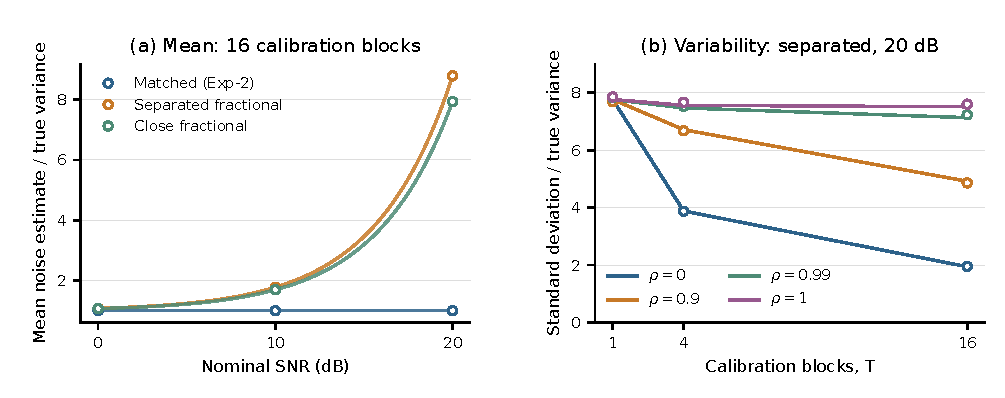
\includegraphics[width=\linewidth]{calibration_bias.pdf}
\caption{Residual-noise calibration. (a) Empirical 16-block means (markers,
15\,000 groups per condition) and analytical expectations (curves).
(b) Empirical relative standard deviations (markers, 20\,000 groups per
correlation condition) and Gaussian predictions (lines joining the evaluated
block counts), for the separated fractional profile at 20~dB. Correlation
acts on the leaked channel energy; the mean remains biased at every block count.}
\label{fig:calibration}
\end{figure}

The gain from pooling depends strongly on temporal correlation. In the separate
correlation audit, the measured relative standard deviation at $T=16$ is
1.955 for independent gains, 4.861 for $\rho=0.9$, 7.235 for $\rho=0.99$,
and 7.605 for constant gains. The corresponding analytical values are
1.942, 4.920, 7.135, and 7.513. The observations agree with the separate
receiver-noise and channel-leakage terms in \eqref{eq:varianceparts}.
Thus the benefit of a 16-block window depends on its temporal spacing and
gain correlation.

For the integer EB receiver, increasing residual pooling from one to 16 blocks
in the separated fractional 20~dB case improves NMSE by 0.047~dB
(pointwise 95\% interval [0.029, 0.064]~dB), while BER increases by 0.00067
(95\% interval [0.00050, 0.00083]).
A residual estimate can thus become sharply concentrated while a substantial
reconstruction error floor remains.

\subsection{Delay offset, subspace width, and useful averaging}
\label{sec:operatingregion}
A prespecified sensitivity study varies the pilot count, delay offset, and
integer-window length. It uses $N=64$, $M\in\{16,32\}$ equally spaced pilots,
delays $(0,7+\delta,11+\delta)$, powers $(0.5,0.3,0.2)$,
$\delta=0,0.1,\ldots,0.9$, and $L=12,13,14,15$.
The 160 combinations of geometry and SNR (10 and 20~dB) are evaluated
analytically for $T=1,4,16$. Independent Monte Carlo checks use 20\,000 groups
per condition at 20~dB for both pilot counts, $L=12,15$, and
$\delta=0,0.2,0.5,0.9$. The complete grid and group estimates are archived.

Figure~\ref{fig:operatingregion} shows how the crossover changes with the
channel geometry. Here normalized calibration MSE means
$\mathbb E[(\widehat v_T-v)^2]/v^2$, distinct from the full-channel NMSE in
Eq.~\eqref{eq:nmse}. At $M=16$, $\delta=0.5$, and 20~dB, increasing $L$ from
12 to 15 reduces $b/v$ from 40.79 to 5.00 and normalized calibration MSE
at $T=16$ from 1765.78 to 27.24. The corresponding $T_\star$ values are
0.98 and 1.44 blocks: both estimates are bias-dominated well before 16
independent blocks. With 32 pilots, the same window change reduces normalized
MSE from 333.46 to 7.31. Across the 48 Monte Carlo checks (16 conditions,
three block counts), means and mean-square errors differ from their predictions
by at most 2.91 and 2.79 Monte Carlo standard errors; sample variances differ
by at most 3.02\%.

\begin{figure}[t]
\centering
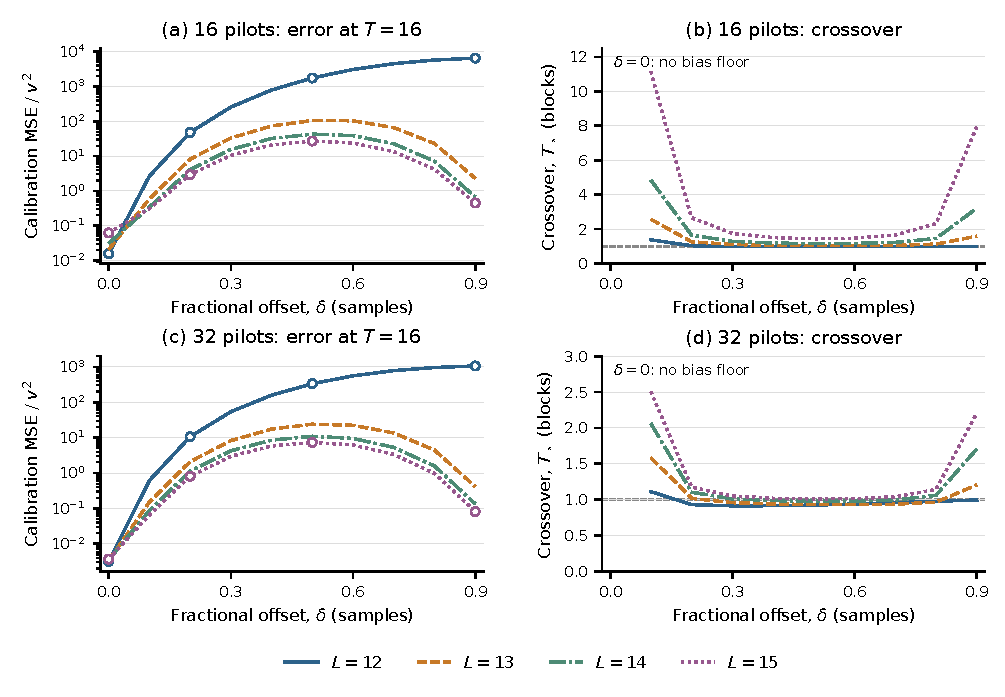
\includegraphics[width=\linewidth]{operating_region.pdf}
\caption{Geometry and window sensitivity at 20~dB with independent gains.
Left: normalized calibration MSE at $T=16$; curves give the analytical
grid and open circles the Monte Carlo checks for $L=12,15$ (20\,000 groups
per condition). Right: the bias--variance crossover $T_\star$ for nonzero
offsets. At $\delta=0$, the channel lies in every tested subspace and there
is no finite crossover. The dashed horizontal reference marks one block.
Lines connect evaluated offsets; the full archive also contains 10~dB and
$T=1,4$ results.}
\label{fig:operatingregion}
\end{figure}

Wider windows reduce both raw leakage and normalized bias at every fractional
offset in this grid, but the calibration MSE also depends on the remaining
residual dimensions. At $M=16$, $\delta=0.1$, and 10~dB, changing $L$ from
12 to 15 lowers $b/v$ from 0.157 to 0.043 while increasing normalized MSE
at $T=16$ from 0.0465 to 0.0698. The intermediate choice $L=13$ gives
0.0292, the smallest MSE among the four tested widths in this condition.
For the matched integer case, the same
change increases MSE from $1/64$ to $1/16$. Thus a wider window is beneficial
when the leakage reduction compensates for the variance cost. The crossover
and MSE quantify that trade-off for the specified channel family and noise level.


\subsection{Confirmation with cyclic-prefix calibration}
The paired CP experiment changes the received calibration samples while
keeping the receiver, its search settings, and the target channel and pilot
realization fixed. It uses the existing CP and its useful-symbol counterparts.
Figure~\ref{fig:cp} shows all four prespecified conditions. CP noise ratios range
from 0.9999 to 1.0069, with relative standard deviations 0.121--0.129,
consistent with the predicted value 0.125. At 20~dB, the corresponding
residual ratios are 8.781 and 7.882 for separated and close fractional paths.

\begin{figure}[t]
\centering
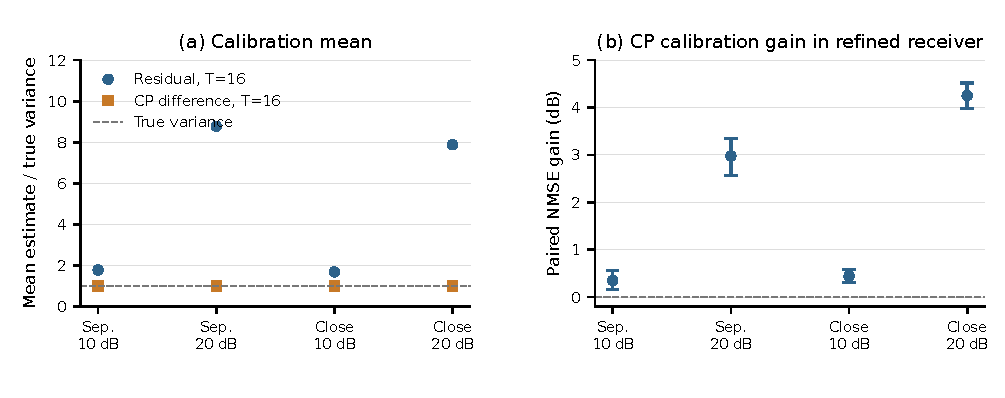
\includegraphics[width=\linewidth]{cp_confirmation.pdf}
\caption{Independent CP-control experiment: 900 groups per cell from three
new seeds. (a) Noise-calibration ratios. (b) NMSE gain obtained by replacing
16-block pilot-residual calibration with 16-block CP calibration in the
same refined receiver. Error bars are pointwise 95\% paired bootstrap
intervals from 2000 resamples. CP and FFT noise retain their physical dependence.}
\label{fig:cp}
\end{figure}

For separated paths at 20~dB, the refined receiver changes from $-21.76$~dB
with residual calibration to $-24.74$~dB with CP calibration; the paired
gain is 2.98~dB [2.57, 3.34]. For close paths, it changes from $-19.15$
to $-23.41$~dB, a gain of 4.25~dB [3.97, 4.52]. BER changes from 0.01000
to 0.00662 and from 0.01206 to 0.00756, respectively. The remaining NMSE
differences from the known-noise controls are 0.10 and 0.04~dB. At 10~dB,
CP gains are smaller, 0.35~dB [0.16, 0.56] and 0.44~dB [0.30, 0.59],
consistent with the smaller leakage-to-noise ratio.

The integer EB receiver gains 0.82 and 0.84~dB at 20~dB on the
same observations. Its CP-calibrated NMSE remains $-13.93$ and $-13.66$~dB.
The smaller gain leaves a substantial representation-dependent error.
In the continuous receiver, the mean selected order
rises from 2.73 to 3.11 for separated paths and from 2.99 to 3.86 for close
paths when CP calibration replaces residual calibration. The changes are
consistent with the residual estimate suppressing weaker components through
the score in \eqref{eq:bic}. These statistics describe the selected orders
as receiver decisions rather than estimates of an exactly identified path count.

The main calibration contrast is stable under an increased optimization
budget: rerunning the flagged fits changes each primary 20~dB CP gain by less
than $10^{-4}$~dB. The original setting selected a candidate at its evaluation
limit in 121 of 10\,800 refined fits; four such cases remained after the budget
extensions. Appendix~\ref{app:optimizer} gives the full diagnostic counts.

\subsection{Representation and calibration have distinct effects}
Figure~\ref{fig:reconstruction} and Table~\ref{tab:reconstruction} compare the
controls for full-channel reconstruction. In the separated fractional 20~dB
case, extending the integer window improves NMSE from $-13.11$ to $-14.43$~dB. Continuous-delay
fitting with the original pooled residual statistic reaches $-22.36$~dB,
a paired gain of 7.93~dB over the extended EB control (95\% interval
[7.54, 8.38]~dB). Supplying the true noise variance to the same continuous
receiver improves NMSE further to $-25.07$~dB. Changing the representation
removes much of the error, but contaminated calibration still affects
model-order selection.

\begin{figure}[t]
\centering
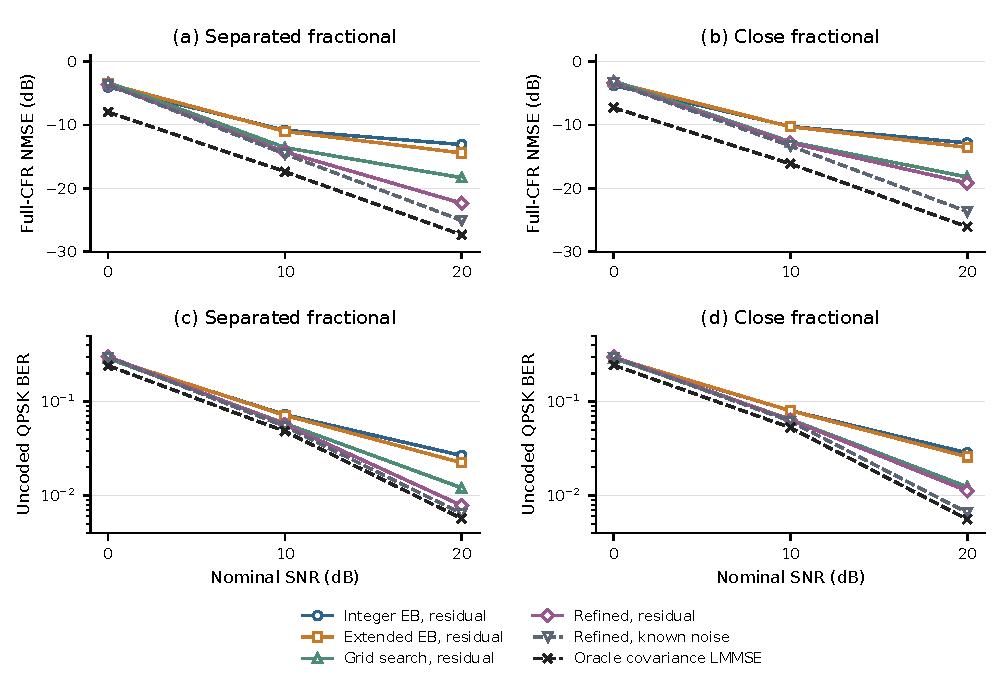
\includegraphics[width=\linewidth]{reconstruction.pdf}
\caption{Exploratory full-channel reconstruction and uncoded detection with
900 paired groups per cell. Residual controls use 16 calibration blocks;
the extended integer control computes its own one-dimensional residual.
The grid and refined controls have different order penalties. Known noise
and exact-covariance LMMSE are explicitly identified information-rich references.}
\label{fig:reconstruction}
\end{figure}

\begin{table}[t]
\centering
\caption{Full-channel NMSE (dB) at 20~dB nominal SNR; 900 paired groups per profile. Integer EB, extended EB, and grid/refined residual controls use 16-block calibration. The known-noise and oracle columns receive extra statistical information.}
\label{tab:reconstruction}
\small\setlength{\tabcolsep}{4pt}
\begin{tabular}{lrrrrrr}
\toprule
& Integer & Extended & Grid & Refined & Refined & Oracle \\
Profile & EB & EB & residual & residual & known $v$ & LMMSE \\
\midrule
Exp-2 & -21.16 & -20.91 & -13.65 & -15.55 & -15.55 & -21.54 \\
Exp-8 & -21.13 & -20.88 & -9.09 & -9.94 & -9.94 & -21.29 \\
Sparse integer & -25.25 & -24.66 & -24.87 & -25.28 & -25.31 & -27.57 \\
Separated fractional & -13.11 & -14.43 & -18.34 & -22.36 & -25.07 & -27.35 \\
Close fractional & -12.84 & -13.55 & -18.23 & -19.19 & -23.67 & -26.06 \\
\bottomrule
\end{tabular}
\end{table}

The gap is larger for the closely spaced profile, where the refined residual
control gives $-19.19$~dB and the known-noise version $-23.67$~dB.
The dense profiles favor the integer subspace. The six-path refined control
gives $-15.55$ and $-9.94$~dB for Exp-2 and Exp-8, whereas integer EB gives
$-21.16$ and $-21.13$~dB. The path cap is below the 12 generating paths in
these cases. The dense-profile comparison is therefore specific to this
six-path fit and its selection and optimization settings. Continuous-delay models can also represent dense
channels through a richer virtual channel impulse response, as demonstrated
by Hansen et al.\ \cite{hansen2018iterative}.

\subsection{Joint inference with a continuous probabilistic model}
Joint continuous-parameter inference provides a second route to separating
signal and noise. We evaluate a Python implementation of VALSE Heuristic~2
from the paper equations \cite{badiu2017valse}, retaining frequency and gain
uncertainty in the noise update. VALSE learns from one target block over a
circular frequency support, while the refined control uses the delay bound
$[0,12]$ and 16 calibration blocks for its residual statistic. The comparison
therefore measures pilot-domain reconstruction and inferred noise under these
different resources. Full-channel interpolation would additionally require a
physical delay branch for the frequency posterior.

Three new seeds give 450 paired groups for each of three sparse profiles
at 10 and 20~dB. The primary setting uses a 500-iteration limit and a relative
reconstruction-change tolerance of $10^{-6}$. All 2700 outputs are retained:
2688 met the stopping criterion, and 12 reached the iteration limit.
Appendix~\ref{app:valse} details the implementation and numerical checks.
Replaying the 12 capped inputs with a 5000-iteration ceiling gives 11 further
convergences. Across the six cells, pilot NMSE changes by at most
0.000624~dB and the mean inferred-noise ratio by $2.72\times10^{-5}$.
The primary table retains the original 500-iteration outputs.

\begin{table}[t]
\centering
\caption{Pilot-domain reconstruction and noise inference; 450 groups per cell. Columns 3--6 give NMSE in dB. VALSE learns noise from one block with circular frequency support; refined controls use the delay bound $[0,12]$. The comparison concerns the observed pilot grid.}
\label{tab:valse}
\small\setlength{\tabcolsep}{4pt}
\begin{tabular}{lrrrrrr}
\toprule
& SNR & Integer & Refined & Refined & VALSE & VALSE \\
Profile & (dB) & EB & residual & known $v$ & & $\mathbb E[\widehat v]/v$ \\
\midrule
Sparse integer & 10 & -14.86 & -14.44 & -14.55 & -14.30 & 1.04 \\
Sparse integer & 20 & -24.98 & -24.86 & -24.86 & -23.86 & 1.13 \\
Separated fractional & 10 & -10.95 & -14.09 & -14.57 & -14.46 & 1.04 \\
Separated fractional & 20 & -13.76 & -22.13 & -24.97 & -23.92 & 1.17 \\
Close fractional & 10 & -10.75 & -12.76 & -13.24 & -12.97 & 1.12 \\
Close fractional & 20 & -13.82 & -18.92 & -23.83 & -19.85 & 1.94 \\
\bottomrule
\end{tabular}
\end{table}

Table~\ref{tab:valse} shows noise inference with a continuous probabilistic
model. At 20~dB, the mean noise ratios were 1.13, 1.17, and 1.94 for integer,
separated fractional, and close fractional paths, respectively. The larger
close-pair ratio accompanies a larger pilot reconstruction error, identifying
a condition where the specified joint inference retains appreciable calibration
error. For separated fractional paths, pilot NMSE was $-23.92$~dB,
between the residual-calibrated and known-noise refined controls. These
pilot-domain observations complement the full-channel CP intervention by
showing how calibration also depends on the inferential model.


\CoreDiscussion

\section{Conclusion}
Residual calibration has a quantifiable transition from sampling-dominated
to leakage-dominated error. For independent blocks, its mean-square error
is $b^2+A/T$, so $T_\star=A/b^2$ for $b>0$ marks equal contributions from squared bias
and variance. Correlated gains change the leakage-fluctuation term and the
useful averaging window. The geometry sweep demonstrates the associated
subspace trade-off: reducing leakage can cost residual dimensions and increase
finite-window error near a matched, low-SNR setting.

The paired receiver experiment establishes the consequence of changing the
noise source. With target pilots and the continuous-delay receiver held
fixed, the established CP statistic improves NMSE by 2.98 and 4.25~dB at
20~dB for the two fractional profiles and recovers most of their known-noise
performance. Integer EB retains a larger representation error on the same
observations. These results provide a model-conditioned basis for choosing
between additional averaging, signal-cancelling calibration, and a more
suitable channel representation.

\appendix
\section{Variational implementation and numerical sensitivity}
\label{app:valse}

The VALSE implementation follows Heuristic~2 and the paper equations
\cite{badiu2017valse}. Sorting the signed pilot frequencies gives a uniformly
spaced sequence indexed by $m=0,\ldots,15$; the constant phase from the
frequency origin is absorbed into each complex gain. The pilot-domain
posterior mean is evaluated at these integer indices. Von Mises moments retain
frequency uncertainty, and the noise update includes gain covariance and
frequency-response uncertainty. Interpolation to noninteger indices requires
an explicit physical delay branch, which lies outside the reported pilot-domain
comparison.

The covariance term uses the paper's global component index; a
source-compatible indexing option is available for inspection. Tests compare
moments with independent numerical quadrature and support-update covariances
with direct matrix inversions. The Python paper-equation implementation has
not been verified for numerical equivalence with the original MATLAB code.
Across the 2700 primary outputs, no run activated noise/prior variance-floor
or Schur-denominator clipping. The implementation documentation records the
high-concentration moment approximation and nonconcave frequency-update
fallback. The differing support restrictions, observation budgets, posterior
approximations, and stopping rules define the scope of the model comparison.

The 12 runs reaching the 500-iteration ceiling were replayed at the
5000-iteration ceiling used in the original VALSE simulation protocol
\cite{badiu2017valse}. Re-execution at 500 iterations first reproduced their
saved outputs. Eleven capped runs then met the stopping criterion, bringing
the total to 2699 of 2700; the remaining run was retained. The largest
converged iteration count among these replays was 1140. The persistent capped
case was a separated fractional profile at 10~dB (seed 1220261115,
group index 19, zero-based).
Using the original complete cell denominators, the largest absolute change
in pilot NMSE was 0.000624~dB and that in mean noise ratio was
$2.72\times10^{-5}$. These sensitivity results support the stability of the
reported cell averages to the iteration ceiling. The main table uses the
original 500-iteration setting throughout.

\section{Continuous-delay optimization sensitivity}
\label{app:optimizer}
The bounded continuous-delay optimizer was checked at increased evaluation
budgets. In a separate 600-call exploratory audit across all five
profiles, 22 selected candidates reached the 60-evaluation limit; 20 of
these occurred in dense profiles. Raising the budget to 300 resolved
18 of the 22 selected-candidate failures. This check assessed the control
under a finite computation budget.

The independent CP experiment recorded diagnostics for all 10\,800 refined
fits. In 782 fits, at least one candidate reached the original evaluation
limit; 121 selected a candidate with that status. Rerunning all 782 flagged
fits with a 300-evaluation limit reduced selected-candidate failures to 18.
Increasing the limit to 1000 for those 18 left four failures. Every estimate
remained finite, and the two primary 20~dB CP-versus-residual gains changed
by less than $10^{-4}$~dB. Re-execution reproduced the original noise arrays
and flagged fits; unflagged per-group metrics were unchanged. The principal
calibration contrast was stable under this budget check, with four residual
stopping failures and possible local minima. The primary results retain the
original predeclared 60-evaluation setting; the sensitivity analysis evaluates
budget dependence rather than certifying a global optimum.



\section*{Data and code availability}
All observations in this study are simulated. The accompanying local
reproducibility package contains the generators, estimator implementations,
random seeds, per-group metric arrays, aggregate numerical results, and figure
scripts. The provenance of the original third-party VALSE demo is documented;
the demo is not redistributed in the package.

\section*{CRediT authorship contribution statement}
Yuxiao Kuang: Conceptualization, Methodology, Software, Formal analysis,
Validation, Visualization, Writing -- original draft, Writing -- review
\& editing. Wenqing Liu: Validation, Formal analysis, Writing -- review
\& editing. Wenjie Li: Validation, Visualization, Writing -- review
\& editing.

\section*{Funding}
This research received no specific grant from funding agencies in the public,
commercial, or not-for-profit sectors.

\section*{Declaration of competing interest}
The authors declare no competing interests.

\section*{Declaration of generative AI and AI-assisted technologies in the manuscript preparation process}
OpenAI Codex was used for debugging assistance.
The authors reviewed and verified the scientific content, code, results,
references, and final text and take full responsibility for the content of
the published article.

\bibliography{references}
\end{document}
